%% Doc Props
\documentclass[11pt,a4paper]{article}
\usepackage[utf8]{inputenc}
\usepackage[english]{babel}

% Packages
\usepackage{
  amsmath,
  titlesec,
  tikz,
  pifont,
  textcomp,
  fixltx2e,
  xcolor,
  fullpage,
  graphicx,
  afterpage,
  lastpage,
  float,
  fancyhdr,
  parskip,
  xfrac,
  gensymb,
  caption,
  subcaption,
  mathtools,
  pdfpages,
  etoolbox,
  enumitem,
  hyperref
}
\usepackage[nottoc,section,numbib]{tocbibind}
%\usepackage[europeancurrents,europeanvoltages,europeanresistors,europeaninductors,smartlabels]{circuitikz}
%\usepackage{pgfplotstable}
%\pgfplotsset{compat=1.12}
\usetikzlibrary{calc,matrix,positioning,arrows,shapes,trees,plotmarks,decorations.markings,shapes.geometric}
\usepackage[font={small,it}]{caption} %% Italics in captions
\tikzstyle{vecArrow} = [thick, decoration={markings,mark=at position 1 with {\arrow[semithick, fill=green]{triangle 60}}}, double distance=1.4pt, shorten >= 5.5pt, preaction = {decorate}, postaction = {draw,line width=1.4pt, green,shorten >= 4.5pt}]
\tikzstyle{innerWhite} = [semithick, green,line width=1.4pt, shorten >= 4.5pt]

\tikzset{
  treenode/.style = {align=center, inner sep=0pt, text centered,font=\sffamily},
  arnn/.style = {treenode, circle, white, font=\sffamily\bfseries, draw=black,fill=black, text width=1.5em},
  arnr/.style = {treenode, circle, red, draw=red, text width=1.5em, very thick},
  arnx/.style = {treenode, rectangle, draw=black,  minimum width=0.5em, minimum height=0.5em}
}

% PDF props
\hypersetup {
  bookmarks=true,              % show bookmarks bar?
  unicode=true,                % non-Latin characters in Acrobat’s bookmarks
  pdftoolbar=true,             % show Acrobat’s toolbar?
  pdfmenubar=true,             % show Acrobat’s menu?
  pdffitwindow=false,          % window fit to page when opened
  pdfstartview={FitH},         % fits the width of the page to the window
  pdftitle={Lab2},                 % title
  pdfauthor={Oscar Petersson}, % author
  pdfsubject={},          % subject of the document
  pdfkeywords={}          % list of keywords
  pdfnewwindow=true,           % links in new window
  hidelinks,                   % hide links (removing color and border)
  linktoc=all,                 % parts of TOC made into links    
}
\urlstyle{same}

% More Props
\graphicspath{{./fig/}}

% Comfy Command Redefinitions
\newcommand{\bve}{\begin{verbatim}}
\newcommand{\itb}{\begin{itemize}}
\newcommand{\ite}{\end{itemize}}
\newcommand{\tb}{\textbackslash}

%% First Page Information
\author{Oscar Petersson, Johan Levinsson}
\title{TDDC17 Lab3}
\date{\today}
\newcommand{\course}{Artificial Intelligence}
\newcommand{\coursenumber}{TDDC17, Linköpings universitet}
\newcommand{\programme}{Högskoleingenjörsutbildning i datateknik, 180 hp}
\newcommand{\examiner}{Josef Fagerström}
\newcommand{\institution}{IDA}
\newcommand{\reptype}{Laboration report}

%%% Document %%%
\begin{document}

\setcounter{secnumdepth}{-1}
\setcounter{tocdepth}{-1}

% Custom titlepage, empty backside, do not use with \maketitle
\pagestyle{empty}
  \makeatletter\begin{center}~\vfill
  \Large{\@author}\vskip .3cm
  \textbf{\LARGE{\@title}}\vskip .2cm
  \large{\programme}
  \vfill
\end{center}
\reptype{} - \@date\hfill Assistant:\\
\textbf{\course}\hfill\examiner\\
\coursenumber\hfill\institution
\makeatother
\newpage
\pagestyle{plain}
%% Table of Contents
%\addtocontents{toc}{\protect\hypertarget{toc}{}}
%\tableofcontents\label{sec:toc}
%\addtocontents{toc}{\protect\thispagestyle{empty}}
%\cleardoublepage
% Call First File Branch
%\section{Q1.}
\em In the vacuum cleaner domain in part 1, what were the states and actions? What is the branching factor?\em

\emph{A1.} Actions: Removing a node from [frontier].\\
    States: Positions in the grid\\
    Branching factor: 4 - maximal possible numbers of branches from a node.\\

\section{Q2.}
\em What is the difference between Breadth First Search and Uniform Cost Search in a domain where the cost
    of each action is 1?\em

\emph{A2.} The implementation (FIFO queue vs priority queue). They behave in the same way though when the cost
    is constant (e.g. the domain given in the question).

\section{Q3.}
\em Suppose that h1 and h2 are admissible heuristics (used in for example A*). Which of the following are
    also admissible?\\
    a) $(h1+h2)/2$\\
    b) $2h1$\\
    c) $\max(h1,h2)$\em

\emph{A3.} (a) and (c)

\section{Q4.}
\em If one would use A* to search for a path to one specific square in the vacuum domain, what could the
    heuristic (h) be? The cost function (g)? Is it an admissible heuristic?\em

\emph{A4.}
    $(h)$: $\sqrt{\Delta{}x\Delta{}y}$ where $\Delta{}\{x,y\}$ is the absolute distance from current
    position to target in the axis (euclidian distance) is one possible heuristic which will always
    underestimate the distance. The manhattan/taxicab distance $|\Delta x| + |\Delta y|$ is another
    possible heuristic which in the given domain never will overestimate and most often underestimate.
    Both are admissable in the given domain.\\
    $(g)$: Any non-descending function. The depth of the node in the current search tree is a sensible option.

\section{Q5.}
\em Draw and explain. Choose your three favorite search algorithms and apply them to any problem domain
    it might be a good idea to use a domain where you can identify a good heuristic function). Draw the
    search tree for them, and explain how they proceed in the searching. Also include the memory usage.
    You can attach a hand-made drawing.\em

    \emph{A5.} Drawing included on page \pageref{fig:a51}. Memory usage is implicitly expressed in the number
    of nodes mapped in the search tree.
     \begin{figure}[h]
  \definecolor{c1}{RGB}{191,255,191}
  \definecolor{c2}{RGB}{127,255,127}
  \definecolor{c3}{RGB}{64,191,64}
  \definecolor{c4}{RGB}{32,127,32}
  %
  \begin{subfigure}[b]{.5\textwidth}
    \centering
    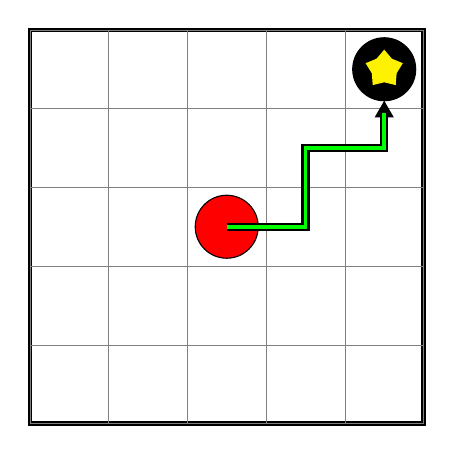
\begin{tikzpicture}
      \draw[black,ultra thick](0,0)rectangle(5,5);
      \draw[step=1cm,gray,very thin] (0,0) grid (5,5);
      \draw[black,fill=black] (4.5,4.5) circle (.4cm) node[star, star points=5,black,fill=yellow] {};
      \draw[black,fill=red] (2.5,2.5) circle (.4cm);
      \draw[vecArrow](2.5,2.5)-|(3.5,3.5)-|(4.5,4.1);
    \end{tikzpicture}
    \caption{A* Search: search through maze}
    \label{fig:a51}
    %
  \end{subfigure}
  %
  \begin{subfigure}[b]{.5\textwidth}
    \centering
    \begin{tikzpicture}[x=.5cm]
      \draw[arrows={-latex}](3,4.25) to [bend right=45] (2,3.75);
      \draw[arrows={-latex}](2,3.25) to [bend right=45] (1,2.75);
      \draw[arrows={-latex}](1,2.25) to [bend left=45] (2,1.75);
      \draw[arrows={-latex}](2,1.25) to [bend left=45] (3,0.75);
      
      \draw[black,fill=red] (3,4.5) ellipse (.35cm and .25cm) node{\textbf{0}};
      
      \draw[black,fill=c1] (2,3.5) ellipse (.35cm and .25cm) node{\textbf{1}};
      \draw[black,fill=lightgray] (4,3.5) ellipse (.35cm and .25cm);

      \draw[black,fill=c1] (1,2.5) ellipse (.35cm and .25cm) node{\textbf{2}};
      \draw[black,fill=lightgray] (3,2.5) ellipse (.35cm and .25cm);
      \draw[black,fill=lightgray] (5,2.5) ellipse (.35cm and .25cm);

      \draw[black,fill=lightgray] (0,1.5) ellipse (.35cm and .25cm);
      \draw[black,fill=c1] (2,1.5) ellipse (.35cm and .25cm) node{\textbf{3}};
      \draw[black,fill=lightgray] (4,1.5) ellipse (.35cm and .25cm);
      \draw[black,fill=lightgray] (6,1.5) ellipse (.35cm and .25cm);

      \draw[black,fill=lightgray] (-1, .5) ellipse (.35cm and .25cm);
      \draw[black,fill=lightgray] (1, .5) ellipse (.35cm and .25cm);
      \draw[yellow,fill=black] (3, .5) ellipse (.35cm and .25cm) node{\textbf{4}};
      \draw[black,fill=lightgray] (5, .5) ellipse (.35cm and .25cm);
      \draw[black,fill=lightgray] (7, .5) ellipse (.35cm and .25cm);
    \end{tikzpicture}
    \caption{A* Search: search tree, 15 nodes}
    \label{fig:a52}
    %
  \end{subfigure}


  \begin{subfigure}[b]{.5\textwidth}
    \centering
    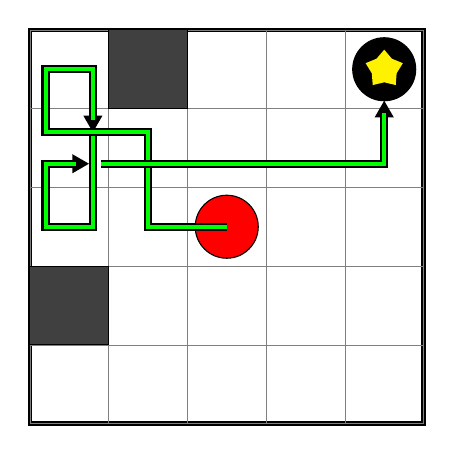
\begin{tikzpicture}
      \draw[black,ultra thick](0,0)rectangle(5,5);
      \draw[step=1cm,gray,very thin] (0,0) grid (5,5);
      \draw[fill=darkgray] (0,1) rectangle (1,2);
      \draw[fill=darkgray] (1,4) rectangle (2,5);
      \draw[black,fill=black] (4.5,4.5) circle (.4cm) node[star, star points=5,black,fill=yellow] {};
      \draw[black,fill=red] (2.5,2.5) circle (.4cm);
      \draw[vecArrow](2.5,2.5)-|(1.5,3.7)-|(.2,4.5)-|(.8,3.7);
      \draw[vecArrow](.8,3.65)|-(.2,2.5)|-(.75,3.3);
      \draw[vecArrow](.9,3.3)-|(4.5,4.1);
    \end{tikzpicture}
    \caption{DFS: search through maze}
    \label{fig:a53}
    %
  \end{subfigure}
  %
  \begin{subfigure}[b]{.5\textwidth}
    \centering
    \begin{tikzpicture}
      \draw[white](0,5.5) circle(.1cm);
      \draw[arrows={-latex}](3,4.25) to [bend right=45] (2.5,3.75);%0-1
      \draw[arrows={-latex}](2.5,3.25) to [bend right=45] (2,2.75);%1-2
      \draw[arrows={-latex}](1.65,2.5) to [bend right=45] (1,1.75); %2-3
      \draw[arrows={-latex}](1,1.25)  to [bend left=45] (0.35,.5);  %3-4,5
      \draw[arrows={-latex}](0.0,0.75) to [bend left=45]  (.65,1.5); %4,5-3
      \draw[arrows={-latex}](1,1.25) to [bend right=45]  (1.65,.5);   %3-6,7
      \draw[arrows={-latex}](2,.75) to [bend right=45]  (1.35,1.5);  %6,7-3
      \draw[arrows={-latex}](1.35,1.5) to [bend right=45]  (2,2.25);  %3-2
      \draw[arrows={-latex}](2.35,2.5) to [bend left=25] (3.5,1.75);  %2-8
      \draw[arrows={-latex}] (3.5,1.25) to [bend left=45] (4,.75);%8-9
      \draw[arrows={-latex}] (4,.25) to [bend left=45] (4.5,-.25);%9-10
      \draw[arrows={-latex}] (4.5,-.75) to [bend left=45] (5,-1.25);%10-11
      \draw[arrows={-latex}] (5,-1.75) to [bend left=45] (5.5,-2.25);%11-12
      
      \draw[black,fill=red] (3,4.5) ellipse (.35cm and .25cm) node{\textbf{0}};      
      \draw[black,fill=c1] (2.5,3.5) ellipse (.35cm and .25cm) node{\textbf{1}};
      \draw[black,fill=c1] (2,2.5) ellipse (.35cm and .25cm) node{\textbf{2,9}};
      \draw[black,fill=c1] (1,1.5) ellipse (.35cm and .25cm) node{\textbf{3,8}};
      \draw[black,fill=c1] (0,0.5) ellipse (.35cm and .25cm) node{\textbf{4,5}};
      \draw[black,fill=c1] (2,0.5) ellipse (.35cm and .25cm) node{\textbf{6,7}};
      \draw[black,fill=c1] (3.5,1.5) ellipse (.35cm and .25cm) node{\textbf{9}};
      \draw[black,fill=c1] (4,0.5) ellipse (.35cm and .25cm) node{\textbf{10}};
      \draw[black,fill=c1] (4.5,-.5) ellipse (.35cm and .25cm) node{\textbf{11}};
      \draw[black,fill=lightgray] (3.5,-.5) ellipse (.35cm and .25cm) node{\textbf{}};
      \draw[black,fill=lightgray] (5.5,-.5) ellipse (.35cm and .25cm) node{\textbf{}};
      \draw[black,fill=c1] (5,-1.5) ellipse (.35cm and .25cm) node{\textbf{12}};
      \draw[black,fill=lightgray] (4,-1.5) ellipse (.35cm and .25cm) node{\textbf{}};
      \draw[black,fill=lightgray] (3,-1.5) ellipse (.35cm and .25cm) node{\textbf{}};
      \draw[black,fill=lightgray] (6,-1.5) ellipse (.35cm and .25cm) node{\textbf{}};
      \draw[yellow,fill=black] (5.5, -2.5) ellipse (.35cm and .25cm) node{\textbf{13}};
    \end{tikzpicture}
    \caption{DFS: search tree, 16 nodes}
    \label{fig:a54}
    %
  \end{subfigure}

  %
  \begin{subfigure}[b]{.4\textwidth}
    \centering
    \begin{tikzpicture}
      \draw[white](0,6.5) circle(.1cm);
      \draw[step=1cm,gray,very thin] (0,0) grid (5,5);
      
      \draw[fill=c4]   (0,0)rectangle(1,1) node[pos=.5] {\textbf{21}};      
      \draw[fill=c3]   (1,0)rectangle(2,1) node[pos=.5] {\textbf{14}};      
      \draw[fill=c2]   (2,0)rectangle(3,1) node[pos=.5] {\textbf{6}};      
      \draw[fill=c3]   (3,0)rectangle(4,1) node[pos=.5] {\textbf{15}};      
      \draw[fill=c4]   (4,0)rectangle(5,1) node[pos=.5] {\textbf{22}};      
      \draw[fill=c3]   (0,1)rectangle(1,2) node[pos=.5] {\textbf{13}};      
      \draw[fill=c2]   (1,1)rectangle(2,2) node[pos=.5] {\textbf{5}};      
      \draw[fill=c1]   (2,1)rectangle(3,2) node[pos=.5] {\textbf{1}};      
      \draw[fill=c2]   (3,1)rectangle(4,2) node[pos=.5] {\textbf{7}};      
      \draw[fill=c3]   (4,1)rectangle(5,2) node[pos=.5] {\textbf{16}};      
      \draw[fill=c2]   (0,2)rectangle(1,3) node[pos=.5] {\textbf{12}};      
      \draw[fill=c1]   (1,2)rectangle(2,3) node[pos=.5] {\textbf{4}};      
      \draw[fill=white](2,2)rectangle(3,3) node[pos=.5] {\textbf{0}};      
      \draw[fill=c1]   (3,2)rectangle(4,3) node[pos=.5] {\textbf{2}};      
      \draw[fill=c2]   (4,2)rectangle(5,3) node[pos=.5] {\textbf{8}};      
      \draw[fill=c3]   (0,3)rectangle(1,4) node[pos=.5] {\textbf{20}};      
      \draw[fill=c2]   (1,3)rectangle(2,4) node[pos=.5] {\textbf{11}};      
      \draw[fill=c1]   (2,3)rectangle(3,4) node[pos=.5] {\textbf{3}};      
      \draw[fill=c2]   (3,3)rectangle(4,4) node[pos=.5] {\textbf{9}};      
      \draw[fill=c3]   (4,3)rectangle(5,4) node[pos=.5] {\textbf{17}};      
      \draw[fill=white](0,4)rectangle(1,5) node[pos=.5] {\textbf{}};      
      \draw[fill=c3]   (1,4)rectangle(2,5) node[pos=.5] {\textbf{19}};      
      \draw[fill=c2]   (2,4)rectangle(3,5) node[pos=.5] {\textbf{10}};      
      \draw[fill=c3]   (3,4)rectangle(4,5) node[pos=.5] {\textbf{18}};      
      \draw[fill=c4]   (4,4)rectangle(5,5) node[pos=.5] {\textbf{23}};      

      \draw[black,fill=red] (2.5,2.5) circle (.4cm) node{\textbf{0}};
      \draw[black,ultra thick](0,0)rectangle(5,5);
      \draw[black,fill=black] (4,4) rectangle (5,5) node[pos=.5,yellow] {\textbf{23}};

    \end{tikzpicture}
    \caption{BFS: search tree, 24 nodes}
    \label{fig:a55}
    %
  \end{subfigure}
  %
  \begin{subfigure}[b]{.6\textwidth}
    \centering
    \begin{tikzpicture}[x=1.0cm]
      \draw[black,fill=red] (6,4.5) ellipse (.35cm and .25cm) node {\textbf{0}};

      \draw[black,fill=c1] (2.75, 3) ellipse (.35cm and .25cm) node {\textbf{1}};
      \draw[black,fill=c1] (6, 3) ellipse (.35cm and .25cm) node {\textbf{2}};
      \draw[black,fill=c1] (8.50, 3) ellipse (.35cm and .25cm) node {\textbf{3}};
      \draw[black,fill=c1] (10.5, 3) ellipse (.35cm and .25cm) node {\textbf{4}};

      \draw[black,fill=c2] (1.5, 2) ellipse (.35cm and .25cm) node {\textbf{5}};
      \draw[black,fill=c2] (3.0, 2) ellipse (.35cm and .25cm) node {\textbf{6}};
      \draw[black,fill=c2] (4.0, 2) ellipse (.35cm and .25cm) node {\textbf{7}};
      \draw[black,fill=c2] (5.5, 2) ellipse (.35cm and .25cm) node {\textbf{8}};
      \draw[black,fill=c2] (6.5, 2) ellipse (.35cm and .25cm) node {\textbf{9}};
      \draw[black,fill=c2] (8.0, 2) ellipse (.35cm and .25cm) node {\textbf{10}};
      \draw[black,fill=c2] (9.0, 2) ellipse (.35cm and .25cm) node {\textbf{11}};
      \draw[black,fill=c2] (10.5,2) ellipse (.35cm and .25cm) node {\textbf{12}};

      \draw[black,fill=c3] (1.0, 1) ellipse (.35cm and .25cm) node {\textbf{13}};
      \draw[black,fill=c3] (2.0, 1) ellipse (.35cm and .25cm) node {\textbf{14}};
      \draw[black,fill=c3] (3.0, 1) ellipse (.35cm and .25cm) node {\textbf{15}};
      \draw[black,fill=c3] (4.0, 1) ellipse (.35cm and .25cm) node {\textbf{16}};
      \draw[black,fill=c3] (5.5, 1) ellipse (.35cm and .25cm) node {\textbf{17}};
      \draw[black,fill=c3] (6.5, 1) ellipse (.35cm and .25cm) node {\textbf{18}};
      \draw[black,fill=c3] (8.0, 1) ellipse (.35cm and .25cm) node {\textbf{19}};
      \draw[black,fill=c3] (9.0, 1) ellipse (.35cm and .25cm) node {\textbf{20}};

      \draw[black,fill=c4] ( 1, 0) ellipse (.35cm and .25cm) node {\textbf{21}};
      \draw[black,fill=c4] ( 3, 0) ellipse (.35cm and .25cm) node {\textbf{22}};
      \draw[yellow,fill=black] (5.5, 0) ellipse (.35cm and .25cm) node {\textbf{23}};

      \draw (6,4.25) to (6,4.12);
      \draw[arrows={-latex}] (6,4.12) to [bend right=10] (2.75,3.25);
      \draw[arrows={-latex}] (6,4.12) to (6,3.25);
      \draw[arrows={-latex}] (6,4.12) to [bend left=10] (8.5,3.25);
      \draw[arrows={-latex}] (6,4.12) to [bend left=10] (10.5,3.25);

      \draw[arrows={-latex}] (2.75,2.75) to [bend right=10] (1.5,2.25);
      \draw[arrows={-latex}] (2.75,2.75) to [bend left=10]  (3,2.25);
      \draw[arrows={-latex}] (2.75,2.75) to [bend left=10]  (4,2.25);

      \draw[arrows={-latex}] (6,2.75) to [bend right=10] (5.5,2.25);
      \draw[arrows={-latex}] (6,2.75) to [bend left=10]  (6.5,2.25);

      \draw[arrows={-latex}] (8.5,2.75) to [bend right=10] (8,2.25);
      \draw[arrows={-latex}] (8.5,2.75) to [bend left=10]  (9,2.25);

      \draw[arrows={-latex}] (10.5,2.75) to (10.5,2.25);

      \draw[arrows={-latex}] (1.5,1.75) to [bend right=10] (1,1.25);
      \draw[arrows={-latex}] (1.5,1.75) to [bend left=10]  (2,1.25);

      \draw[arrows={-latex}] (3,1.75) to (3,1.25);

      \draw[arrows={-latex}] (4,1.75) to (4,1.25);

      \draw[arrows={-latex}] (5.5,1.75) to (5.5,1.25);

      \draw[arrows={-latex}] (6.5,1.75) to (6.5,1.25);

      \draw[arrows={-latex}] (8,1.75) to (8,1.25);

      \draw[arrows={-latex}] (9,1.75) to (9,1.25);

      \draw[arrows={-latex}] (1,0.75) to (1,0.25);

      \draw[arrows={-latex}] (3,0.75) to (3,0.25);

      \draw[arrows={-latex}] (5.5,0.75) to (5.5,0.25);




      
    \end{tikzpicture}
    \caption{BFS: search tree}
    \label{fig:a56}
    %
  \end{subfigure}

    
\end{figure}


\section{Q6.}
\em Look at all the offline search algorithms presented in chapter 3 plus A* search. Are they complete?
    Are they optimal? Explain why!\em

    \emph{A6.}
    
    \begin{tabular}{l|c|c}
      Algorithm & Complete & Optimal \\
      \hline
      Breadth-First & Yes & Yes \\
      Depth-First & No & No\\
      Iterative-Deepening & Yes & Yes\\
      Bidirectional & BFS & No\\
      Greedy Best First & Graph & No\\
      A* & Yes & Yes      
    \end{tabular}

    BFS is complete if the branching factor is finite and there is a solution, and it is optimal if the cost
    is a non-decreasing function.

    DFS is incomplete as it can get stuck in infinite branches.

    Iterative Deepening Search is complete if the branching factor is finite, and it is optimal if the cost is
    a non-decreasing function.

    Bidirectional Search is implementation (DFS or BFS) dependent regarding completeness. It is not optimal
    since the path found needs to be verified optimal.

    For Greedy BFS, tree search is incomplete as it can get stuck in dead-end branches, but graph search is
    complete thanks to keeping track of explored noted.

    A* is complete. It requires the existence of a finite number of paths where the cost equals that of the
    optimal path. It is optimal if the heuristic function is admissable.
    
\section{Q7.}
\em Assume that you had to go back and do Lab 1/Task 2 once more (if you did not use search already).
    Remember that the agent did not have perfect knowledge of the environment but had to explore it
    incrementally. Which of the search algorithms you have learned would be most suited in this situation
    to guide the agent's execution? What would you search for? Give an example.\em

    \emph{A7.}
    We did use search (BFS), even though either one could do the work in the given domain. The objective
    would be to find that something doesn't exist in the domain, i.e. accessible unexplored nodes.

\section{Q1.}
\em In the vacuum cleaner domain in part 1, what were the states and actions? What is the branching factor?\em

\emph{A1.} Actions: Removing a node from [frontier].\\
    States: Positions in the grid\\
    Branching factor: 4 - maximal possible numbers of branches from a node.\\

\section{Q2.}
\em What is the difference between Breadth First Search and Uniform Cost Search in a domain where the cost
    of each action is 1?\em

\emph{A2.} The implementation (FIFO queue vs priority queue). They behave in the same way though when the cost
    is constant (e.g. the domain given in the question).

\section{Q3.}
\em Suppose that h1 and h2 are admissible heuristics (used in for example A*). Which of the following are
    also admissible?\\
    a) $(h1+h2)/2$\\
    b) $2h1$\\
    c) $\max(h1,h2)$\em

\emph{A3.} (a) and (c)

\section{Q4.}
\em If one would use A* to search for a path to one specific square in the vacuum domain, what could the
    heuristic (h) be? The cost function (g)? Is it an admissible heuristic?\em

\emph{A4.}
    $(h)$: $\sqrt{\Delta{}x\Delta{}y}$ where $\Delta{}\{x,y\}$ is the absolute distance from current
    position to target in the axis (euclidian distance) is one possible heuristic which will always
    underestimate the distance. The manhattan/taxicab distance $|\Delta x| + |\Delta y|$ is another
    possible heuristic which in the given domain never will overestimate and most often underestimate.
    Both are admissable in the given domain.\\
    $(g)$: Any non-descending function. The depth of the node in the current search tree is a sensible option.

\section{Q5.}
\em Draw and explain. Choose your three favorite search algorithms and apply them to any problem domain
    it might be a good idea to use a domain where you can identify a good heuristic function). Draw the
    search tree for them, and explain how they proceed in the searching. Also include the memory usage.
    You can attach a hand-made drawing.\em

    \emph{A5.} Drawing included on page \pageref{fig:a51}. Memory usage is implicitly expressed in the number
    of nodes mapped in the search tree.
     \begin{figure}[h]
  \definecolor{c1}{RGB}{191,255,191}
  \definecolor{c2}{RGB}{127,255,127}
  \definecolor{c3}{RGB}{64,191,64}
  \definecolor{c4}{RGB}{32,127,32}
  %
  \begin{subfigure}[b]{.5\textwidth}
    \centering
    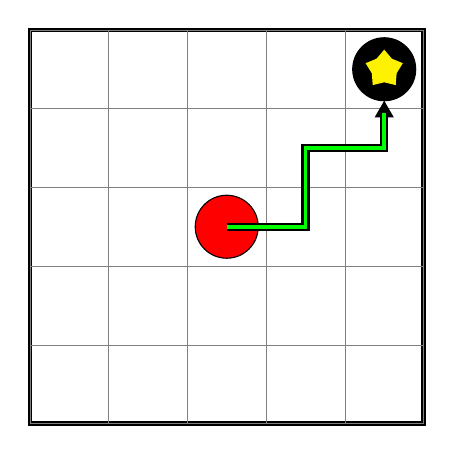
\begin{tikzpicture}
      \draw[black,ultra thick](0,0)rectangle(5,5);
      \draw[step=1cm,gray,very thin] (0,0) grid (5,5);
      \draw[black,fill=black] (4.5,4.5) circle (.4cm) node[star, star points=5,black,fill=yellow] {};
      \draw[black,fill=red] (2.5,2.5) circle (.4cm);
      \draw[vecArrow](2.5,2.5)-|(3.5,3.5)-|(4.5,4.1);
    \end{tikzpicture}
    \caption{A* Search: search through maze}
    \label{fig:a51}
    %
  \end{subfigure}
  %
  \begin{subfigure}[b]{.5\textwidth}
    \centering
    \begin{tikzpicture}[x=.5cm]
      \draw[arrows={-latex}](3,4.25) to [bend right=45] (2,3.75);
      \draw[arrows={-latex}](2,3.25) to [bend right=45] (1,2.75);
      \draw[arrows={-latex}](1,2.25) to [bend left=45] (2,1.75);
      \draw[arrows={-latex}](2,1.25) to [bend left=45] (3,0.75);
      
      \draw[black,fill=red] (3,4.5) ellipse (.35cm and .25cm) node{\textbf{0}};
      
      \draw[black,fill=c1] (2,3.5) ellipse (.35cm and .25cm) node{\textbf{1}};
      \draw[black,fill=lightgray] (4,3.5) ellipse (.35cm and .25cm);

      \draw[black,fill=c1] (1,2.5) ellipse (.35cm and .25cm) node{\textbf{2}};
      \draw[black,fill=lightgray] (3,2.5) ellipse (.35cm and .25cm);
      \draw[black,fill=lightgray] (5,2.5) ellipse (.35cm and .25cm);

      \draw[black,fill=lightgray] (0,1.5) ellipse (.35cm and .25cm);
      \draw[black,fill=c1] (2,1.5) ellipse (.35cm and .25cm) node{\textbf{3}};
      \draw[black,fill=lightgray] (4,1.5) ellipse (.35cm and .25cm);
      \draw[black,fill=lightgray] (6,1.5) ellipse (.35cm and .25cm);

      \draw[black,fill=lightgray] (-1, .5) ellipse (.35cm and .25cm);
      \draw[black,fill=lightgray] (1, .5) ellipse (.35cm and .25cm);
      \draw[yellow,fill=black] (3, .5) ellipse (.35cm and .25cm) node{\textbf{4}};
      \draw[black,fill=lightgray] (5, .5) ellipse (.35cm and .25cm);
      \draw[black,fill=lightgray] (7, .5) ellipse (.35cm and .25cm);
    \end{tikzpicture}
    \caption{A* Search: search tree, 15 nodes}
    \label{fig:a52}
    %
  \end{subfigure}


  \begin{subfigure}[b]{.5\textwidth}
    \centering
    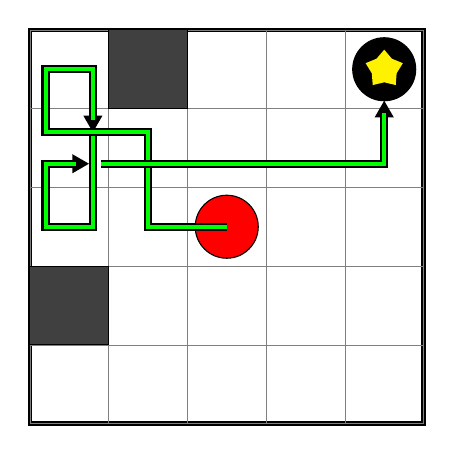
\begin{tikzpicture}
      \draw[black,ultra thick](0,0)rectangle(5,5);
      \draw[step=1cm,gray,very thin] (0,0) grid (5,5);
      \draw[fill=darkgray] (0,1) rectangle (1,2);
      \draw[fill=darkgray] (1,4) rectangle (2,5);
      \draw[black,fill=black] (4.5,4.5) circle (.4cm) node[star, star points=5,black,fill=yellow] {};
      \draw[black,fill=red] (2.5,2.5) circle (.4cm);
      \draw[vecArrow](2.5,2.5)-|(1.5,3.7)-|(.2,4.5)-|(.8,3.7);
      \draw[vecArrow](.8,3.65)|-(.2,2.5)|-(.75,3.3);
      \draw[vecArrow](.9,3.3)-|(4.5,4.1);
    \end{tikzpicture}
    \caption{DFS: search through maze}
    \label{fig:a53}
    %
  \end{subfigure}
  %
  \begin{subfigure}[b]{.5\textwidth}
    \centering
    \begin{tikzpicture}
      \draw[white](0,5.5) circle(.1cm);
      \draw[arrows={-latex}](3,4.25) to [bend right=45] (2.5,3.75);%0-1
      \draw[arrows={-latex}](2.5,3.25) to [bend right=45] (2,2.75);%1-2
      \draw[arrows={-latex}](1.65,2.5) to [bend right=45] (1,1.75); %2-3
      \draw[arrows={-latex}](1,1.25)  to [bend left=45] (0.35,.5);  %3-4,5
      \draw[arrows={-latex}](0.0,0.75) to [bend left=45]  (.65,1.5); %4,5-3
      \draw[arrows={-latex}](1,1.25) to [bend right=45]  (1.65,.5);   %3-6,7
      \draw[arrows={-latex}](2,.75) to [bend right=45]  (1.35,1.5);  %6,7-3
      \draw[arrows={-latex}](1.35,1.5) to [bend right=45]  (2,2.25);  %3-2
      \draw[arrows={-latex}](2.35,2.5) to [bend left=25] (3.5,1.75);  %2-8
      \draw[arrows={-latex}] (3.5,1.25) to [bend left=45] (4,.75);%8-9
      \draw[arrows={-latex}] (4,.25) to [bend left=45] (4.5,-.25);%9-10
      \draw[arrows={-latex}] (4.5,-.75) to [bend left=45] (5,-1.25);%10-11
      \draw[arrows={-latex}] (5,-1.75) to [bend left=45] (5.5,-2.25);%11-12
      
      \draw[black,fill=red] (3,4.5) ellipse (.35cm and .25cm) node{\textbf{0}};      
      \draw[black,fill=c1] (2.5,3.5) ellipse (.35cm and .25cm) node{\textbf{1}};
      \draw[black,fill=c1] (2,2.5) ellipse (.35cm and .25cm) node{\textbf{2,9}};
      \draw[black,fill=c1] (1,1.5) ellipse (.35cm and .25cm) node{\textbf{3,8}};
      \draw[black,fill=c1] (0,0.5) ellipse (.35cm and .25cm) node{\textbf{4,5}};
      \draw[black,fill=c1] (2,0.5) ellipse (.35cm and .25cm) node{\textbf{6,7}};
      \draw[black,fill=c1] (3.5,1.5) ellipse (.35cm and .25cm) node{\textbf{9}};
      \draw[black,fill=c1] (4,0.5) ellipse (.35cm and .25cm) node{\textbf{10}};
      \draw[black,fill=c1] (4.5,-.5) ellipse (.35cm and .25cm) node{\textbf{11}};
      \draw[black,fill=lightgray] (3.5,-.5) ellipse (.35cm and .25cm) node{\textbf{}};
      \draw[black,fill=lightgray] (5.5,-.5) ellipse (.35cm and .25cm) node{\textbf{}};
      \draw[black,fill=c1] (5,-1.5) ellipse (.35cm and .25cm) node{\textbf{12}};
      \draw[black,fill=lightgray] (4,-1.5) ellipse (.35cm and .25cm) node{\textbf{}};
      \draw[black,fill=lightgray] (3,-1.5) ellipse (.35cm and .25cm) node{\textbf{}};
      \draw[black,fill=lightgray] (6,-1.5) ellipse (.35cm and .25cm) node{\textbf{}};
      \draw[yellow,fill=black] (5.5, -2.5) ellipse (.35cm and .25cm) node{\textbf{13}};
    \end{tikzpicture}
    \caption{DFS: search tree, 16 nodes}
    \label{fig:a54}
    %
  \end{subfigure}

  %
  \begin{subfigure}[b]{.4\textwidth}
    \centering
    \begin{tikzpicture}
      \draw[white](0,6.5) circle(.1cm);
      \draw[step=1cm,gray,very thin] (0,0) grid (5,5);
      
      \draw[fill=c4]   (0,0)rectangle(1,1) node[pos=.5] {\textbf{21}};      
      \draw[fill=c3]   (1,0)rectangle(2,1) node[pos=.5] {\textbf{14}};      
      \draw[fill=c2]   (2,0)rectangle(3,1) node[pos=.5] {\textbf{6}};      
      \draw[fill=c3]   (3,0)rectangle(4,1) node[pos=.5] {\textbf{15}};      
      \draw[fill=c4]   (4,0)rectangle(5,1) node[pos=.5] {\textbf{22}};      
      \draw[fill=c3]   (0,1)rectangle(1,2) node[pos=.5] {\textbf{13}};      
      \draw[fill=c2]   (1,1)rectangle(2,2) node[pos=.5] {\textbf{5}};      
      \draw[fill=c1]   (2,1)rectangle(3,2) node[pos=.5] {\textbf{1}};      
      \draw[fill=c2]   (3,1)rectangle(4,2) node[pos=.5] {\textbf{7}};      
      \draw[fill=c3]   (4,1)rectangle(5,2) node[pos=.5] {\textbf{16}};      
      \draw[fill=c2]   (0,2)rectangle(1,3) node[pos=.5] {\textbf{12}};      
      \draw[fill=c1]   (1,2)rectangle(2,3) node[pos=.5] {\textbf{4}};      
      \draw[fill=white](2,2)rectangle(3,3) node[pos=.5] {\textbf{0}};      
      \draw[fill=c1]   (3,2)rectangle(4,3) node[pos=.5] {\textbf{2}};      
      \draw[fill=c2]   (4,2)rectangle(5,3) node[pos=.5] {\textbf{8}};      
      \draw[fill=c3]   (0,3)rectangle(1,4) node[pos=.5] {\textbf{20}};      
      \draw[fill=c2]   (1,3)rectangle(2,4) node[pos=.5] {\textbf{11}};      
      \draw[fill=c1]   (2,3)rectangle(3,4) node[pos=.5] {\textbf{3}};      
      \draw[fill=c2]   (3,3)rectangle(4,4) node[pos=.5] {\textbf{9}};      
      \draw[fill=c3]   (4,3)rectangle(5,4) node[pos=.5] {\textbf{17}};      
      \draw[fill=white](0,4)rectangle(1,5) node[pos=.5] {\textbf{}};      
      \draw[fill=c3]   (1,4)rectangle(2,5) node[pos=.5] {\textbf{19}};      
      \draw[fill=c2]   (2,4)rectangle(3,5) node[pos=.5] {\textbf{10}};      
      \draw[fill=c3]   (3,4)rectangle(4,5) node[pos=.5] {\textbf{18}};      
      \draw[fill=c4]   (4,4)rectangle(5,5) node[pos=.5] {\textbf{23}};      

      \draw[black,fill=red] (2.5,2.5) circle (.4cm) node{\textbf{0}};
      \draw[black,ultra thick](0,0)rectangle(5,5);
      \draw[black,fill=black] (4,4) rectangle (5,5) node[pos=.5,yellow] {\textbf{23}};

    \end{tikzpicture}
    \caption{BFS: search tree, 24 nodes}
    \label{fig:a55}
    %
  \end{subfigure}
  %
  \begin{subfigure}[b]{.6\textwidth}
    \centering
    \begin{tikzpicture}[x=1.0cm]
      \draw[black,fill=red] (6,4.5) ellipse (.35cm and .25cm) node {\textbf{0}};

      \draw[black,fill=c1] (2.75, 3) ellipse (.35cm and .25cm) node {\textbf{1}};
      \draw[black,fill=c1] (6, 3) ellipse (.35cm and .25cm) node {\textbf{2}};
      \draw[black,fill=c1] (8.50, 3) ellipse (.35cm and .25cm) node {\textbf{3}};
      \draw[black,fill=c1] (10.5, 3) ellipse (.35cm and .25cm) node {\textbf{4}};

      \draw[black,fill=c2] (1.5, 2) ellipse (.35cm and .25cm) node {\textbf{5}};
      \draw[black,fill=c2] (3.0, 2) ellipse (.35cm and .25cm) node {\textbf{6}};
      \draw[black,fill=c2] (4.0, 2) ellipse (.35cm and .25cm) node {\textbf{7}};
      \draw[black,fill=c2] (5.5, 2) ellipse (.35cm and .25cm) node {\textbf{8}};
      \draw[black,fill=c2] (6.5, 2) ellipse (.35cm and .25cm) node {\textbf{9}};
      \draw[black,fill=c2] (8.0, 2) ellipse (.35cm and .25cm) node {\textbf{10}};
      \draw[black,fill=c2] (9.0, 2) ellipse (.35cm and .25cm) node {\textbf{11}};
      \draw[black,fill=c2] (10.5,2) ellipse (.35cm and .25cm) node {\textbf{12}};

      \draw[black,fill=c3] (1.0, 1) ellipse (.35cm and .25cm) node {\textbf{13}};
      \draw[black,fill=c3] (2.0, 1) ellipse (.35cm and .25cm) node {\textbf{14}};
      \draw[black,fill=c3] (3.0, 1) ellipse (.35cm and .25cm) node {\textbf{15}};
      \draw[black,fill=c3] (4.0, 1) ellipse (.35cm and .25cm) node {\textbf{16}};
      \draw[black,fill=c3] (5.5, 1) ellipse (.35cm and .25cm) node {\textbf{17}};
      \draw[black,fill=c3] (6.5, 1) ellipse (.35cm and .25cm) node {\textbf{18}};
      \draw[black,fill=c3] (8.0, 1) ellipse (.35cm and .25cm) node {\textbf{19}};
      \draw[black,fill=c3] (9.0, 1) ellipse (.35cm and .25cm) node {\textbf{20}};

      \draw[black,fill=c4] ( 1, 0) ellipse (.35cm and .25cm) node {\textbf{21}};
      \draw[black,fill=c4] ( 3, 0) ellipse (.35cm and .25cm) node {\textbf{22}};
      \draw[yellow,fill=black] (5.5, 0) ellipse (.35cm and .25cm) node {\textbf{23}};

      \draw (6,4.25) to (6,4.12);
      \draw[arrows={-latex}] (6,4.12) to [bend right=10] (2.75,3.25);
      \draw[arrows={-latex}] (6,4.12) to (6,3.25);
      \draw[arrows={-latex}] (6,4.12) to [bend left=10] (8.5,3.25);
      \draw[arrows={-latex}] (6,4.12) to [bend left=10] (10.5,3.25);

      \draw[arrows={-latex}] (2.75,2.75) to [bend right=10] (1.5,2.25);
      \draw[arrows={-latex}] (2.75,2.75) to [bend left=10]  (3,2.25);
      \draw[arrows={-latex}] (2.75,2.75) to [bend left=10]  (4,2.25);

      \draw[arrows={-latex}] (6,2.75) to [bend right=10] (5.5,2.25);
      \draw[arrows={-latex}] (6,2.75) to [bend left=10]  (6.5,2.25);

      \draw[arrows={-latex}] (8.5,2.75) to [bend right=10] (8,2.25);
      \draw[arrows={-latex}] (8.5,2.75) to [bend left=10]  (9,2.25);

      \draw[arrows={-latex}] (10.5,2.75) to (10.5,2.25);

      \draw[arrows={-latex}] (1.5,1.75) to [bend right=10] (1,1.25);
      \draw[arrows={-latex}] (1.5,1.75) to [bend left=10]  (2,1.25);

      \draw[arrows={-latex}] (3,1.75) to (3,1.25);

      \draw[arrows={-latex}] (4,1.75) to (4,1.25);

      \draw[arrows={-latex}] (5.5,1.75) to (5.5,1.25);

      \draw[arrows={-latex}] (6.5,1.75) to (6.5,1.25);

      \draw[arrows={-latex}] (8,1.75) to (8,1.25);

      \draw[arrows={-latex}] (9,1.75) to (9,1.25);

      \draw[arrows={-latex}] (1,0.75) to (1,0.25);

      \draw[arrows={-latex}] (3,0.75) to (3,0.25);

      \draw[arrows={-latex}] (5.5,0.75) to (5.5,0.25);




      
    \end{tikzpicture}
    \caption{BFS: search tree}
    \label{fig:a56}
    %
  \end{subfigure}

    
\end{figure}


\section{Q6.}
\em Look at all the offline search algorithms presented in chapter 3 plus A* search. Are they complete?
    Are they optimal? Explain why!\em

    \emph{A6.}
    
    \begin{tabular}{l|c|c}
      Algorithm & Complete & Optimal \\
      \hline
      Breadth-First & Yes & Yes \\
      Depth-First & No & No\\
      Iterative-Deepening & Yes & Yes\\
      Bidirectional & BFS & No\\
      Greedy Best First & Graph & No\\
      A* & Yes & Yes      
    \end{tabular}

    BFS is complete if the branching factor is finite and there is a solution, and it is optimal if the cost
    is a non-decreasing function.

    DFS is incomplete as it can get stuck in infinite branches.

    Iterative Deepening Search is complete if the branching factor is finite, and it is optimal if the cost is
    a non-decreasing function.

    Bidirectional Search is implementation (DFS or BFS) dependent regarding completeness. It is not optimal
    since the path found needs to be verified optimal.

    For Greedy BFS, tree search is incomplete as it can get stuck in dead-end branches, but graph search is
    complete thanks to keeping track of explored noted.

    A* is complete. It requires the existence of a finite number of paths where the cost equals that of the
    optimal path. It is optimal if the heuristic function is admissable.
    
\section{Q7.}
\em Assume that you had to go back and do Lab 1/Task 2 once more (if you did not use search already).
    Remember that the agent did not have perfect knowledge of the environment but had to explore it
    incrementally. Which of the search algorithms you have learned would be most suited in this situation
    to guide the agent's execution? What would you search for? Give an example.\em

    \emph{A7.}
    We did use search (BFS), even though either one could do the work in the given domain. The objective
    would be to find that something doesn't exist in the domain, i.e. accessible unexplored nodes.


\end{document}
